\documentclass{article}

% Anonymous double-blind workshop submission.
\usepackage[dblblindworkshop]{neurips_2026}
\workshoptitle{AgenticOS @ NeurIPS 2026}

\usepackage[utf8]{inputenc}
\usepackage[T1]{fontenc}
\usepackage{hyperref}
\usepackage{url}
\usepackage{booktabs}
\usepackage{amsfonts}
\usepackage{amsmath}
\usepackage{nicefrac}
\usepackage{microtype}
\usepackage{xcolor}
\usepackage{graphicx}
\usepackage{multirow}
\usepackage{enumitem}

\newcommand{\hal}{\textsc{hal}}
\newcommand{\nd}{\textsc{nd}}
\newcommand{\rhoS}{\rho}
\newcommand{\tauK}{\tau_b}

\title{Does Cost-Efficiency Travel? Accuracy and Cost Rank Transfer in Fixed-Scaffold Agent Evaluation}

\author{Anonymous Author(s)}

\begin{document}
\maketitle

\begin{abstract}
Agent leaderboards increasingly report both task success and dollar cost, inviting practitioners to select a ``cost-efficient'' model from a single benchmark. We test whether this selection signal transfers across workloads. Using public results from the Holistic Agent Leaderboard (\hal), we hold the displayed agent scaffold fixed to the HAL Generalist Agent and compare repeated displayed model labels across six benchmarks. Accuracy-rank association is often positive across benchmark pairs, while dollar-cost-rank association is markedly more heterogeneous: among pairs with at least 12 shared labels, cost Spearman correlation ranges from $0.74$ to $0.93$; across all eligible pairs it ranges from $-0.75$ to $0.93$. For example, GAIA and ScienceAgentBench have accuracy correlation $0.64$ but cost correlation $-0.75$ over seven shared labels. Correspondingly, nondominated accuracy--cost frontier sets have low overlap. We also distinguish the ordinary nondominated frontier from a HAL-inspired convex-hull reconstruction, finding that the public HAL labels align closely with the latter but not identically. These descriptive results suggest that dollar-cost efficiency from one agent leaderboard should not be presumed portable to another workload, even when accuracy ordering is partly preserved. The study does not identify causal model or scaffold effects: public display labels do not fully encode all benchmark-specific setup details.
\end{abstract}

\section{Introduction}

Agent benchmarks now evaluate systems that reason over multiple steps, invoke tools, and interact with environments. Unlike static model evaluations, an agent's reported behavior depends on an underlying language model, an agent scaffold, tools, prompts, execution limits, and the task environment. These systems can also be expensive to evaluate: the Holistic Agent Leaderboard (\hal) reports 21,730 rollouts across nine benchmarks and roughly \$40,000 in evaluation cost~\citep{kapoor2026hal}. Consequently, cost-aware leaderboards increasingly plot accuracy against dollar cost and recommend points on a cost--accuracy frontier.

A practical inference often follows: if a model or agent is cost-efficient on one benchmark, it is a promising low-cost choice elsewhere. This inference is plausible if model capability and model cost are mostly portable. It can fail if an agent's token consumption, retry loops, tool calls, and stopping behavior change with the workload. This paper asks a narrow descriptive question: \emph{when the publicly displayed scaffold is held fixed, how stable are repeated HAL displayed model labels' accuracy ranks, dollar-cost ranks, and cost--accuracy frontier positions across workloads?}

We conduct a secondary analysis of public HAL leaderboard data. The data are sparse and unbalanced across scaffolds, so rather than attempt an unsupported causal decomposition of model, scaffold, and workload effects, we focus on the only broadly repeated scaffold: the HAL Generalist Agent. Across six benchmarks with sufficient overlap, we compare rankings only among shared displayed model labels. Our main findings are:
\begin{itemize}[leftmargin=*,nosep]
    \item Accuracy-rank associations are often positive, but dollar-cost-rank associations are substantially more heterogeneous and can be negative.
    \item Nondominated cost--accuracy frontier membership is correspondingly unstable: no displayed label tested on at least five of the six workloads is nondominated on every tested workload.
    \item Frontier conclusions depend on the decision model. The public HAL \texttt{Is Pareto} labels closely match an origin-anchored convex-hull reconstruction, whereas standard nondominance retains additional points.
\end{itemize}

The result is not universal non-transfer. Some pairs show high agreement in both accuracy and dollar cost. Rather, transfer cannot safely be assumed from a single leaderboard.

\section{Related work}

\paragraph{Cost-aware agent evaluation.}
\citet{kapoor2026hal} introduced HAL as a standardized, cost-aware agent leaderboard spanning coding, web, science, and customer-service settings. HAL reports dollar- and token-cost Pareto curves and documents substantial scaffold sensitivity. \citet{agentsmatter2024} argue that agent evaluation should jointly consider accuracy and cost, using Pareto plots to expose avoidable expenditure. SWE-Effi studies resource-constrained software-engineering agents and reports that effectiveness depends on scaffold--model integration~\citep{sweeffi2025}. These works establish the importance of cost and scaffold effects, but do not systematically measure whether a cost--accuracy ordering transfers between distinct workloads under a fixed scaffold.

\paragraph{Stability of agent and benchmark rankings.}
\citet{ndzomga2026efficient} ask whether smaller task subsets can preserve \emph{within-benchmark} agent rankings under scaffold and temporal shift. Their target is evaluation reduction, not cross-workload transfer of cost--accuracy trade-offs. In the static-LLM setting, Benchmark$^2$ proposes cross-benchmark ranking consistency based on Kendall correlation~\citep{qian2026benchmark2}. We adapt the cross-benchmark ranking perspective to interactive agents and separately analyze accuracy ranks, dollar-cost ranks, and frontier-set overlap.

\section{Data, scope, and coverage}
\label{sec:data}

We use the public \texttt{all\_leaderboards\_costs\_HAL.csv} snapshot distributed with \citet{ndzomga2026efficient}. The frozen file contains 242 displayed evaluations across nine benchmarks, 11 displayed scaffolds, and 29 displayed model labels. Accuracy and total dollar cost are complete, but 235 rows report a single run and only seven report two runs. The data therefore support descriptive rank and frontier analysis, not rollout-level uncertainty estimation.

Coverage determines the design. Most scaffolds occur on only one benchmark; the HAL Generalist Agent occurs on seven. We retain the six Generalist benchmarks with adequate overlap: CORE-Bench Hard (21 labels), GAIA (17), SciCode (9), ScienceAgentBench (7), SWE-bench Verified Mini (18), and TAU-bench Airline (14). We exclude USACO because it contains one Generalist row. Figure~\ref{fig:coverage} shows the resulting incomplete label-by-benchmark matrix.

\begin{figure}[t]
  \centering
  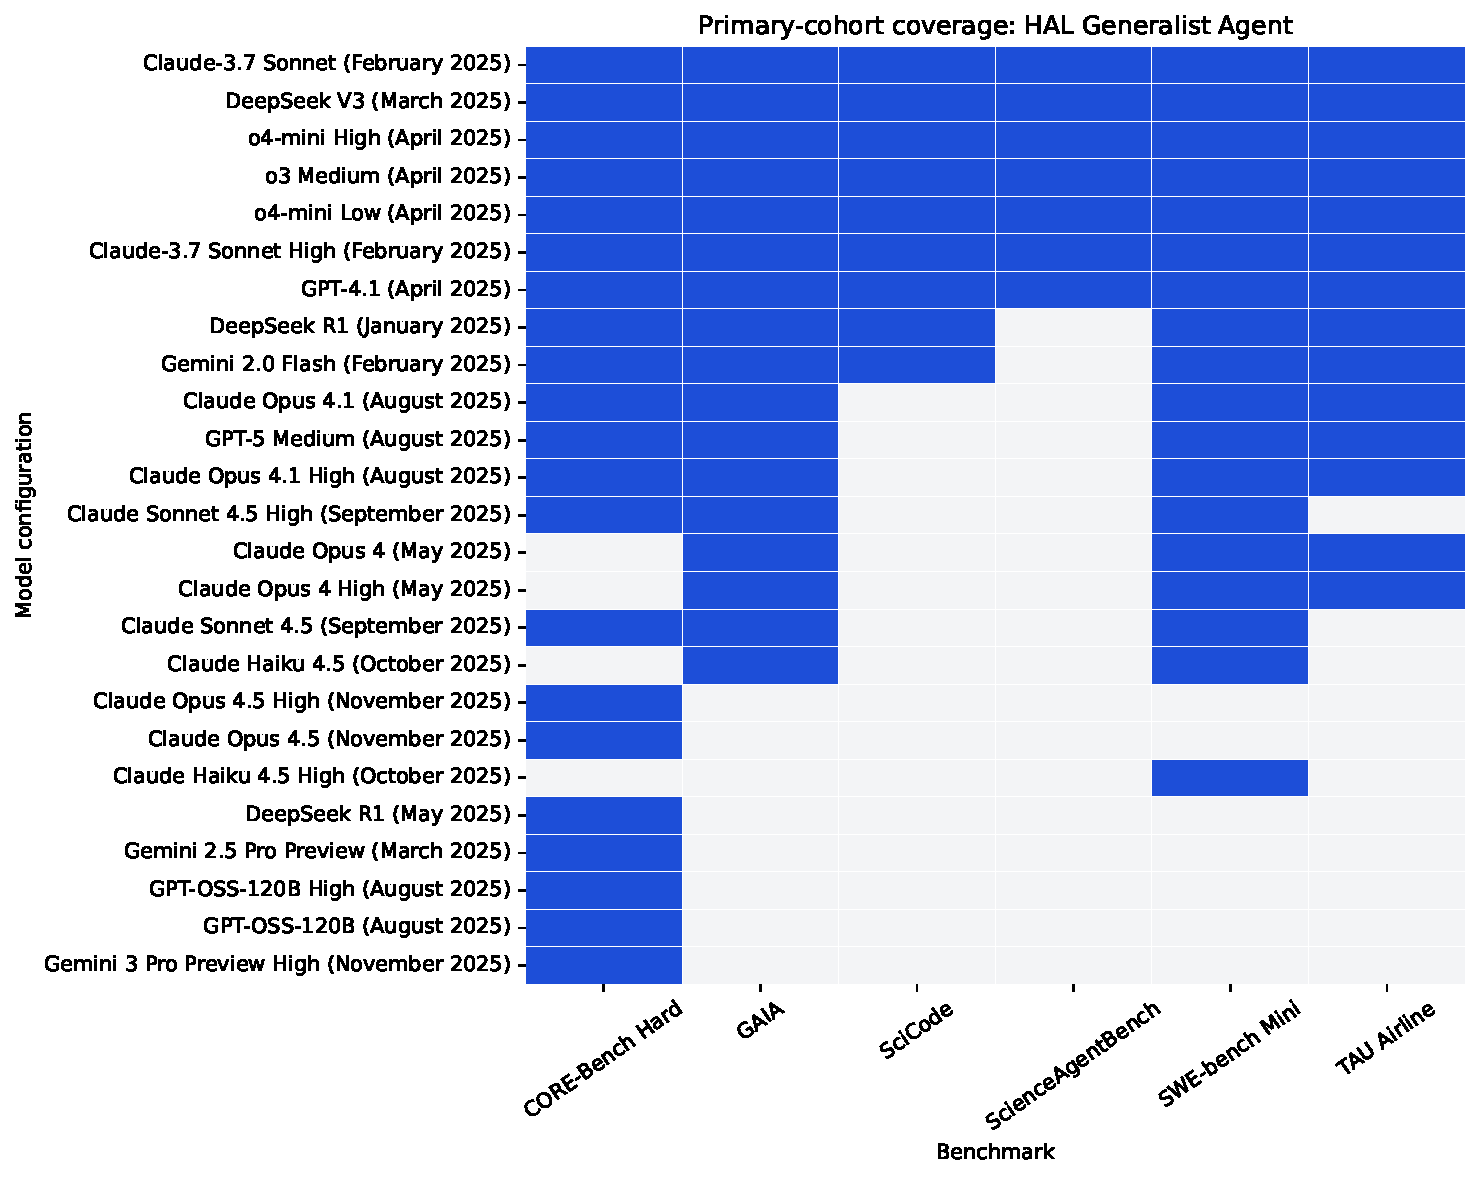
\includegraphics[width=0.94\linewidth]{figures/coverage_heatmap.pdf}
  \caption{Coverage of the primary cohort. A filled cell indicates that the public HAL table contains the displayed model label under the displayed HAL Generalist Agent scaffold. Sparse coverage motivates pairwise analyses restricted to shared labels.}
  \label{fig:coverage}
\end{figure}

The repeated unit is an exact public \texttt{Models} display string within the exact public \texttt{Agent Name} display string. This includes the visible date and reasoning suffix when present. It does \emph{not} fully specify all benchmark-specific prompts, tools, budgets, or harness settings. Thus, the analysis describes repeated public HAL labels under a repeated displayed scaffold; it is not a controlled base-model experiment.

\section{Method}
\label{sec:method}

\paragraph{Rank transfer.}
For each benchmark pair with at least five shared displayed labels, we compute Spearman rank correlation $\rhoS$ and Kendall's $\tauK$ separately for accuracy and total dollar cost. Let $L_{ij}$ be labels observed in both benchmarks $i$ and $j$. We correlate their displayed accuracy values and, separately, their displayed total costs. We report $|L_{ij}|$ for every pair.

To characterize sensitivity to the finite label set, we use 5,000 percentile \emph{configuration-resampling} draws: resample shared labels with replacement and recompute the correlation. These intervals are neither rollout-level uncertainty intervals nor population-model confidence intervals. Degenerate draws without rank variation are excluded and counted. We do not use interval inclusion of zero for hypothesis testing.

\paragraph{Two frontier definitions.}
For lower cost and higher accuracy, the nondominated frontier includes point $x$ if no observed point $y$ has cost no greater than $x$, accuracy at least that of $x$, and at least one strict improvement. This corresponds to choosing one displayed configuration. HAL's public analysis code instead adds the origin and computes an upper cost--accuracy hull, which has a randomized-policy interpretation: a mixture of two systems can dominate an interior point in expectation. We implement a \emph{HAL-inspired convex-hull reconstruction} based on the public reference code, while avoiding a claim of exact identity because two supplied labels differ in this frozen snapshot. For both definitions, we report pairwise Jaccard similarity of frontier sets. We distinguish full-cohort frontiers from frontiers recomputed only on a pair's shared labels.

\paragraph{Scaffold sensitivity.}
As a secondary descriptive check, we compare shared displayed labels across scaffolds \emph{within} a benchmark, reporting paired accuracy differences and log cost ratios. This confirms prior scaffold sensitivity rather than estimating a general scaffold effect.

\section{Results}
\label{sec:results}

\subsection{Accuracy ranks transfer more consistently than dollar-cost ranks}

Figure~\ref{fig:similarity} is the main result. Accuracy-rank correlations are often positive, while cost-rank correlations vary from strongly positive to strongly negative. GAIA--SWE-bench Mini has 17 shared labels and shows positive association in both accuracy ($\rhoS=0.71$) and cost ($\rhoS=0.89$). In contrast, GAIA--ScienceAgentBench has $\rhoS=0.64$ for accuracy but $\rhoS=-0.75$ for dollar cost over seven shared labels. SciCode--SWE-bench Mini is near zero for both metrics ($\rhoS=0.15$ accuracy, $0.02$ cost, $N=9$), but its broad configuration-resampling intervals make it a descriptive example rather than precise evidence of no association.

\begin{figure*}[t]
  \centering
  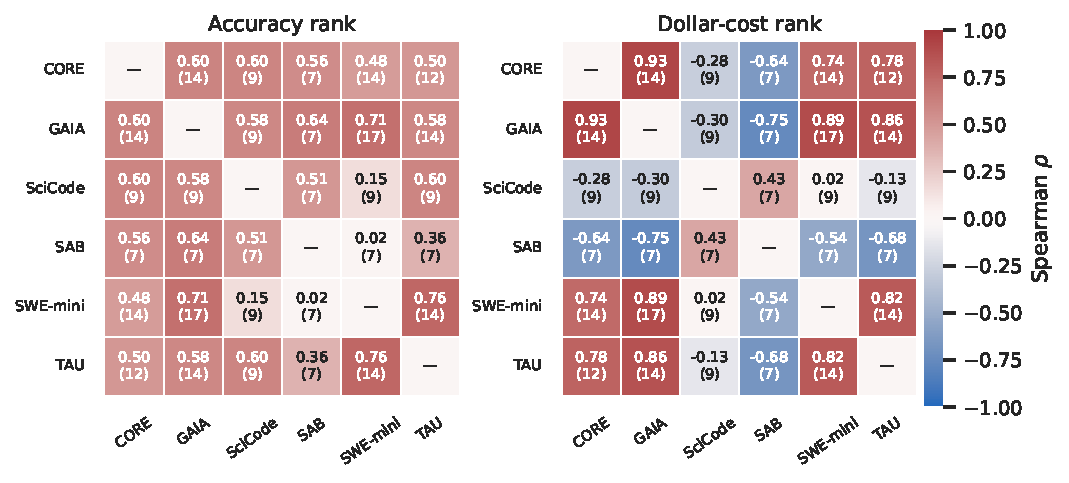
\includegraphics[width=0.98\textwidth]{figures/rank_transfer_compact.pdf}
  \caption{Cross-workload rank transfer under the displayed HAL Generalist Agent scaffold. Each off-diagonal cell reports Spearman $\rhoS$ and the number of shared displayed labels. Accuracy association is often positive, whereas dollar-cost association is more heterogeneous; negative values occur for several pairs involving ScienceAgentBench.}
  \label{fig:similarity}
\end{figure*}

Table~\ref{tab:highoverlap} lists the six pairs with at least 12 shared labels. The strongest evidence comes from these larger-overlap comparisons: cost ranks are highly aligned in these pairs, but nondominated frontier Jaccard similarity remains low to moderate ($0.17$--$0.43$). Thus, even where two scalar ranks agree, binary frontier composition can change as the achievable accuracy--cost trade-off changes.

\begin{table}[t]
\caption{Higher-overlap benchmark pairs. Brackets are 5,000-draw configuration-resampling sensitivity intervals, not rollout-level confidence intervals. ND denotes nondominated frontier membership recomputed on the shared-label cohort.}
\label{tab:highoverlap}
\centering
\footnotesize
\begin{tabular}{lrrrr}
\toprule
Pair & N & Accuracy $\rho$ & Cost $\rho$ & ND Jaccard \\
\midrule
CORE-Bench Hard--GAIA & 14 & 0.60 [0.16, 0.81] & 0.93 [0.72, 0.99] & 0.43 \\
CORE-Bench Hard--SWE-bench Mini & 14 & 0.48 [-0.05, 0.82] & 0.74 [0.29, 0.93] & 0.25 \\
CORE-Bench Hard--TAU Airline & 12 & 0.50 [-0.12, 0.86] & 0.78 [0.26, 0.98] & 0.17 \\
GAIA--SWE-bench Mini & 17 & 0.71 [0.31, 0.91] & 0.89 [0.61, 0.99] & 0.33 \\
GAIA--TAU Airline & 14 & 0.58 [0.14, 0.85] & 0.86 [0.58, 0.97] & 0.29 \\
SWE-bench Mini--TAU Airline & 14 & 0.76 [0.40, 0.91] & 0.82 [0.46, 0.97] & 0.43 \\
\bottomrule
\end{tabular}

\end{table}

\subsection{Frontier membership is not portable}

Figure~\ref{fig:frontier} displays nondominated membership by workload. Among labels tested on at least five workloads, Claude-3.7 Sonnet High has the highest nondominated appearance count, four of six; no broadly tested label is nondominated everywhere. Table~\ref{tab:rates} summarizes the broadly covered labels. Because membership is discontinuous near a frontier, we interpret this result together with the continuous rank results rather than as a standalone universal ranking.

\begin{figure}[t]
  \centering
  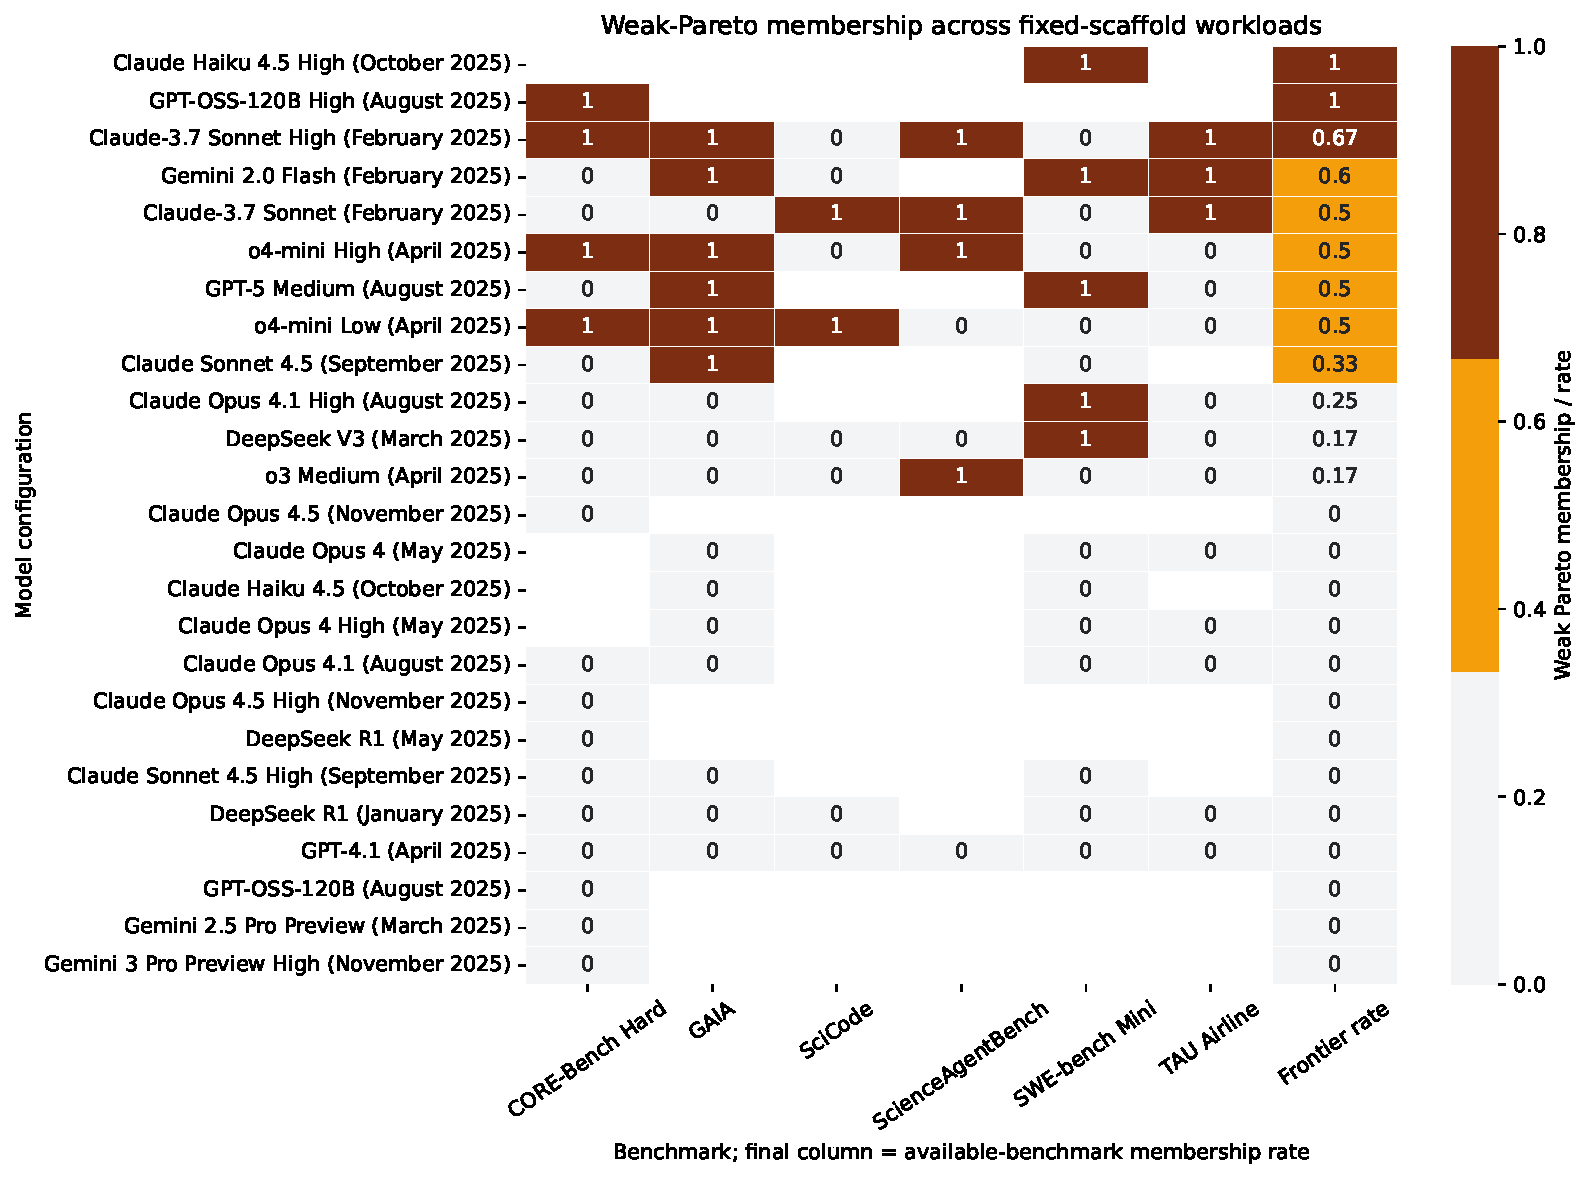
\includegraphics[width=0.98\linewidth]{figures/weak_pareto_membership.pdf}
  \caption{Nondominated cost--accuracy membership across primary workloads. The final column is each label's rate over its available workloads. No label tested on at least five workloads is nondominated on all of them.}
  \label{fig:frontier}
\end{figure}

\begin{table}[t]
\caption{Nondominated frontier appearances for labels tested on at least five primary workloads.}
\label{tab:rates}
\centering
\footnotesize
\begin{tabular}{lrrr}
\toprule
Model label & Tested & ND appearances & ND rate \\
\midrule
Claude-3.7 Sonnet High & 6 & 4 & 0.67 \\
Claude-3.7 Sonnet & 6 & 3 & 0.50 \\
o4-mini High & 6 & 3 & 0.50 \\
o4-mini Low & 6 & 3 & 0.50 \\
DeepSeek V3 & 6 & 1 & 0.17 \\
o3 Medium & 6 & 1 & 0.17 \\
GPT-4.1 & 6 & 0 & 0.00 \\
Gemini 2.0 Flash & 5 & 3 & 0.60 \\
DeepSeek R1 & 5 & 0 & 0.00 \\
\bottomrule
\end{tabular}

\end{table}

\subsection{Frontier definition and scaffold comparisons matter}

The source HAL labels recover 30 frontier rows under the hull reconstruction, with two discrepancies; standard nondominance includes 19 additional non-dominated rows. This is substantively relevant: a discrete buyer choosing one agent and a deployer willing to randomize between agents solve different decision problems.

Within individual benchmarks, scaffold changes are also large and direction-dependent. For example, across 15 shared labels on SWE-bench Mini, the displayed SWE-Agent is on average 27.4 percentage points more accurate than the displayed Generalist scaffold, with a higher median cost. Across seven shared labels on ScienceAgentBench, SAB Self-Debug is both more accurate on average and lower cost. These benchmark-specific contrasts are consistent with HAL and SWE-Effi, and motivate rather than replace the fixed-scaffold primary design.

\section{Discussion}

The practical implication is conditional, not absolute. A cost-efficient point on one benchmark can be a useful prior, especially when benchmark pairs show strong cost-rank agreement. Yet cost rank is not uniformly portable, and several pairs exhibit weak or negative association despite positive accuracy association. Dollar cost plausibly responds to workload-specific execution dynamics---tool calls, retries, loop length, and termination behavior---in addition to model pricing. A practitioner selecting an agent for a new workload should therefore validate cost on representative tasks rather than extrapolate from a single efficiency leaderboard.

The analysis also highlights a reporting issue. A frontier label is not self-explanatory: ordinary nondominance and a convex-hull/randomization frontier encode different deployment choices. Leaderboards should state which decision model they use and, when feasible, expose both.

\section{Limitations}

This is a secondary analysis of a sparse public snapshot. First, repeated coverage is incomplete; most scaffolds occur on only one benchmark, and the primary fixed-scaffold analysis retains only six workloads. Second, public display labels do not fully encode benchmark-specific prompts, tool policies, budgets, or harness versions. Holding a display label fixed does not isolate a causal base-model effect. Third, most evaluations are single-run, so configuration-resampling intervals do not measure rollout variance. Fourth, dollar cost combines observed execution with pricing assumptions; the supplied CSV lacks token totals, preventing a token-cost robustness analysis. Fifth, only three same-domain pairs are available under HAL's categories, so domain conclusions are exploratory and omitted from the main claim. Finally, frontier membership is sensitive to the comparator set and small changes near the frontier; we therefore report both full-cohort and shared-cohort analyses in the supplemental material.

\section{Conclusion}

Across public HAL results with a repeated displayed Generalist scaffold, accuracy ranks often transfer more consistently than dollar-cost ranks, while cost--accuracy frontier membership is not reliably portable. The evidence is heterogeneous rather than uniformly negative: some workload pairs align strongly on both axes. Still, a single benchmark's cost-efficiency ranking is insufficient evidence for selecting an agent on a new workload. Future agent leaderboards should use crossed model--scaffold--benchmark designs with repeated runs and report both token- and dollar-based decision frontiers.

\bibliographystyle{plainnat}
\bibliography{references}

\clearpage
\appendix
\section{Frontier-label reproducibility audit}
\label{app:pareto}
\begin{table}[h]
\caption{Supplied HAL frontier labels compared with reconstructed frontiers by benchmark. Agreement is the fraction of displayed rows with identical Boolean labels.}
\centering
\scriptsize
\begin{tabular}{lrrrrrr}
\toprule
Benchmark & Rows & Supplied & Nondominated & Hull & Supplied--ND agreement & Supplied--hull agreement \\
\midrule
assistantbench & 15 & 2 & 3 & 2 & 0.933 & 1.000 \\
corebench\_hard & 45 & 5 & 10 & 5 & 0.889 & 1.000 \\
gaia & 32 & 4 & 6 & 4 & 0.938 & 1.000 \\
online\_mind2web & 22 & 3 & 4 & 3 & 0.955 & 1.000 \\
scicode & 33 & 2 & 3 & 3 & 0.970 & 0.970 \\
scienceagentbench & 23 & 4 & 8 & 4 & 0.826 & 1.000 \\
swebench\_verified\_mini & 33 & 3 & 7 & 3 & 0.879 & 1.000 \\
taubench\_airline & 26 & 3 & 3 & 4 & 1.000 & 0.962 \\
usaco & 13 & 4 & 5 & 4 & 0.923 & 1.000 \\
\bottomrule
\end{tabular}

\end{table}

\section{Reproducibility details}
The analysis freezes the public CSV using the recorded source hash in the
anonymous supplement. It uses exact public display labels, minimum pairwise overlap five, 5,000
configuration-resampling draws, and random seed 20260816. The released anonymous
supplement should include the analysis code, input provenance manifest, generated
tables, and commands needed to regenerate all figures.

\section*{NeurIPS Paper Checklist}

\begin{enumerate}
\item \textbf{Claims}
    \item[] Question: Do the main claims made in the abstract and introduction accurately reflect the paper's contributions and scope?
    \item[] Answer: \answerYes{}
    \item[] Justification: The abstract and introduction state that the analysis is descriptive, restricted to repeated public HAL display labels under a repeated displayed scaffold, and does not identify causal model or scaffold effects.

\item \textbf{Limitations}
    \item[] Question: Does the paper discuss the limitations of the work performed by the authors?
    \item[] Answer: \answerYes{}
    \item[] Justification: Section~6 discusses sparse coverage, display-label ambiguity, single-run evaluations, price dependence, missing token totals, limited domain comparisons, and frontier sensitivity.

\item \textbf{Theory assumptions and proofs}
    \item[] Question: For each theoretical result, does the paper provide the full set of assumptions and a complete (and correct) proof?
    \item[] Answer: \answerNA{}
    \item[] Justification: The paper presents an empirical secondary analysis and no theoretical results.

\item \textbf{Experimental result reproducibility}
    \item[] Question: Does the paper fully disclose all the information needed to reproduce the main experimental results of the paper to the extent that it affects the main claims and/or conclusions of the paper (regardless of whether the code and data are provided or not)?
    \item[] Answer: \answerYes{}
    \item[] Justification: Sections~3--4 and the appendix specify the public source, frozen hash, inclusion criteria, matching unit, frontier definitions, overlap threshold, resampling procedure, and seed.

\item \textbf{Open access to data and code}
    \item[] Question: Does the paper provide open access to the data and code, with sufficient instructions to faithfully reproduce the main experimental results, as described in supplemental material?
    \item[] Answer: \answerYes{}
    \item[] Justification: An anonymized supplement will contain the analysis code, provenance manifest, and reproduction instructions; the underlying public data source is cited.

\item \textbf{Experimental setting/details}
    \item[] Question: Does the paper specify all the training and test details (e.g., data splits, hyperparameters, how they were chosen, type of optimizer) necessary to understand the results?
    \item[] Answer: \answerYes{}
    \item[] Justification: No models are trained. The data filtering, rank metrics, frontier definitions, resampling count, and seed are specified in Sections~3--4.

\item \textbf{Experiment statistical significance}
    \item[] Question: Does the paper report error bars suitably and correctly defined or other appropriate information about the statistical significance of the experiments?
    \item[] Answer: \answerYes{}
    \item[] Justification: We report configuration-resampling sensitivity intervals and explicitly state that they are not rollout-level or population-model confidence intervals and are not used for hypothesis tests.

\item \textbf{Experiments compute resources}
    \item[] Question: For each experiment, does the paper provide sufficient information on the computer resources (type of compute workers, memory, time of execution) needed to reproduce the experiments?
    \item[] Answer: \answerNA{}
    \item[] Justification: The work is a lightweight secondary analysis of public tabular data and uses no model training or agent rollouts.

\item \textbf{Code of ethics}
    \item[] Question: Does the research conducted in the paper conform, in every respect, with the NeurIPS Code of Ethics \url{https://neurips.cc/public/EthicsGuidelines}?
    \item[] Answer: \answerYes{}
    \item[] Justification: The work uses public aggregate evaluation data, attributes source authors, reports limitations, and makes no claims about people or protected groups.

\item \textbf{Broader impacts}
    \item[] Question: Does the paper discuss both potential positive societal impacts and negative societal impacts of the work performed?
    \item[] Answer: \answerYes{}
    \item[] Justification: We use **Yes** here because the work has practical consequences. Better reporting of success-adjusted cost and execution telemetry can reduce wasted evaluation and deployment spend. Conversely, treating a single leaderboard's dollar ranking as a deployment recommendation can misallocate resources or favor systems whose price/configuration signal does not transfer. The paper's safeguards are explicit claim boundaries, public-data provenance, and reproducible sensitivity analyses.

\item \textbf{Safeguards}
    \item[] Question: Does the paper describe safeguards that have been put in place for responsible release of data or models that have a high risk for misuse (e.g., pre-trained language models, image generators, or scraped datasets)?
    \item[] Answer: \answerNA{}
    \item[] Justification: The paper releases no trained model, agent capability, or new high-risk dataset.

\item \textbf{Licenses for existing assets}
    \item[] Question: Are the creators or original owners of assets (e.g., code, data, models), used in the paper, properly credited and are the license and terms of use explicitly mentioned and properly respected?
    \item[] Answer: \answerYes{}
    \item[] Justification: The data and methodological sources are cited; the supplement records the upstream repository, commit, source path, and declared MIT license.

\item \textbf{New assets}
    \item[] Question: Are new assets introduced in the paper well documented and is the documentation provided alongside the assets?
    \item[] Answer: \answerYes{}
    \item[] Justification: The analysis code and generated tables are documented by a source manifest, artifact manifest, tests, and reproduction commands.

\item \textbf{Crowdsourcing and research with human subjects}
    \item[] Question: For crowdsourcing experiments and research with human subjects, does the paper include the full text of instructions given to participants and screenshots, if applicable, as well as details about compensation (if any)?
    \item[] Answer: \answerNA{}
    \item[] Justification: The study involves no crowdsourcing and no human subjects research.

\item \textbf{Institutional review board (IRB) approvals or equivalent for research with human subjects}
    \item[] Question: Does the paper describe potential risks incurred by study participants, whether such risks were disclosed to the subjects, and whether Institutional Review Board (IRB) approvals (or an equivalent approval/review based on the requirements of your country or institution) were obtained?
    \item[] Answer: \answerNA{}
    \item[] Justification: The study involves no human subjects research.

\item \textbf{Declaration of LLM usage}
    \item[] Question: Does the paper describe the usage of LLMs if it is an important, original, or non-standard component of the core methods in this research?
    \item[] Answer: \answerNA{}
    \item[] Justification: The core method is deterministic analysis of public tabular data; no LLM is used as a component of the empirical method.
\end{enumerate}


\end{document}
